\documentclass{article}

\usepackage[english]{babel}
\usepackage[utf8]{inputenc}
\usepackage{amsmath,amssymb}
\usepackage{parskip}
\usepackage{graphicx}
%\usepackage{subcaption}
\usepackage{amsmath}
\usepackage{float}
\usepackage{mathtools}

\usepackage{subfig}
\usepackage[dvipsnames]{xcolor}
\usepackage[justification=centering]{caption}




% Margins
\usepackage[top=2cm, left=2.5cm, right=2.5cm, bottom=3.0cm]{geometry}
% Colour table cells
%\usepackage[table]{xcolor}

%\colorlet{myBlue}{blue!10!black!10!}
%\colorlet{myBlue}{Violet}
\definecolor{myBlue}{HTML}{0000CC}

% Get larger line spacing in table
\newcommand{\tablespace}{\\[1.25mm]}
\newcommand\Tstrut{\rule{0pt}{2.6ex}}         % = `top' strut
\newcommand\tstrut{\rule{0pt}{2.0ex}}         % = `top' strut
\newcommand\Bstrut{\rule[-0.9ex]{0pt}{0pt}}   % = `bottom' strut


\def\one{\mbox{1\hspace{-4.25pt}\fontsize{12}{14.4}\selectfont\textrm{1}}}

%%%%%%%%%%%%%%%%%
%     Title     %
%%%%%%%%%%%%%%%%%
\title{HPC Project: Parallelizing a multilayer perceptron with openmp}
\author{Marian Aldescu - marian.aldescu@etu.univ-grenoble-alpes.fr}
\date{\today}

\begin{document}
	\maketitle
	
	\begin{abstract}
		Start with a statement regarding the purpose or objective of the assignment.
		
		Summarize your solution to the problem your procedure/design methodology.
		
		Summarize your results
		
		Briefly draw some conclusions based on your results
		
		In general, anyone should be able to read your abstract and get a general idea of what appears in the rest of the report
		
		It might be a good idea to write this section last
		
		
		
	\end{abstract}
	
	
\section{Design Methodology}


\subsection{About the MLP}

The work in this project is based on the first specification of a Multilayer Perceptron(MLP) given in \cite{rumelhart}, which is a method to learn patterns in a set of data, then generalize the rules on unseen samples, probably the most common notion in the field of deep learning.

It is important to keep in mind that the name(\textit{multilayer perceptron}) may be misleading, since it does not use the perceptron algorithm for training, but the backpropagation algorithm. We detail the second later.
	

Let's se what is the idea behind a MLP. For this, we refer to the notion of Artificial Neural Network(ANN), a method of learning inspired by the human brain. An ANN can be imagined as a directed graph, composed of layers, each of them containing a variable number of processing nodes(\textit{neurons}). Normally, nodes in the same layer are not connected between them, but only to nodes in the next layer. Edges are endowed with \textit{weights} and neurons with a \textit{threshold}(bias). First layer's number of nodes should match the size of input data, and the output layer's dimension is 1 or more, depending on the task. In Figure \ref{fig:mlp_1}, such an architecture can be seen.

We need also to mention that the input of a neuron is computed as a linear combination of the neurons outputs from the previous layer, as in the 
following equation:
\begin{eqnarray}
z_k = b_k + \sum_{i=1}^{n}w_{ki}x_i 
\end{eqnarray}

where $x_i \in \mathbb{R}^d$ is a training sample, $z_k$ is the neuron's value after the linear function is applied on it, $b_k$ is the neuron's bias and $w_{ki}$, the weights for all previous layer's neurons.

The interesting part that makes ANNs so powerful is the non-linearity  applied on the neuron's linear function, and it is usually one of the: sigmoid, tanh, ReLU, softmax. They are usually chosen depending on the task at hand. If considering the sigmoid function, the activation($a_k$) looks as in Eq.(2).
\begin{eqnarray}
	a_k = \sigma(z_k) = \frac{1}{1+e^{-z_k}} 
\end{eqnarray}


\begin{figure}[htbp]
	\centering
	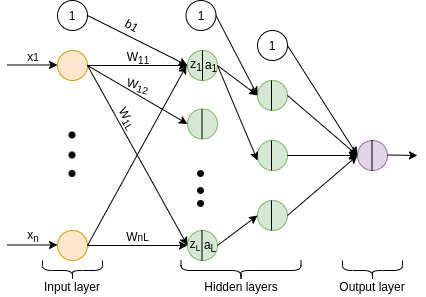
\includegraphics[scale=0.6]{fig/MLP.png}
	\caption{General architecture of a MLP with n inputs, 2 hidden layers and 1 output. One auxiliary node is added per layer to support the bias.}
	\label{fig:mlp_1}
\end{figure}

Another essential aspect and probably the most important one is the cost function, also know as the objective that we want to minimize over the entire data set. There are different cost functions, but as in the original paper\cite{rumelhart}, I used the \textit{sum of squared erros}, shown in Eq.(3), where $y_i$ is the expected label and $f(x_i)$ the predicted value for sample $x_i$. We multiply it with $\frac{1}{2}$, as it will facilitate the computation of the gradient later.
\begin{eqnarray}
	E = \frac{1}{2} \sum_{i=1}^{N}(y_i - f(x_i))
\end{eqnarray}


Now that we have defined the structure of MLP, let's describe the behavior by which the learning happens. It can be split in 2 steps: \textit{forward propagation} and \textit{backward propagation}.\\



\subsection{Forward propagation as a task parallelism model}
It consists of feeding each sample of the data set to the NN, layer by layer, until the last one, when the error is calculated. We saw previously that in a MLP, nodes acts a processing units: they compute the linear function and then, the activation of a neuron, therefore we can see them as small tasks that can be run in parallel(Eq.4), with the mention that only operations of the same layer are able to run at the same time, as one layer depends on the previous layer's computation. Edges of the NN are "streams" of data, which at the same time apply their associated weights on the flow.

\begin{equation}
\text{	Run in parallel }
	\begin{cases}
		z_1 = b_1 + \sum_{i=1}^{n}w_{1i}x_i \\
		...\\
		z_K = b_K + \sum_{i=1}^{n}w_{Ki}x_i 
	\end{cases}       
\iff z = W^\top \times x	
\end{equation}

where $z_1, ..., z_k$ are the values of the neurons in a layer of size $K$, and their computation can be formulated as a matrix multiplication, where $W$ contains the biases of neurons on the first row and $x$ contains value 1 on the first position, then the values of $\vec{x}$.

For a layer, its activations(Eq.5) could also be computed in parallel, but I choose no to do this, as normally it doesn't have a large number of 
neurons(usually, maximum the order of thousands), since the parallelization
\begin{equation}
	a = 
	\begin{bmatrix}
		\sigma(z_1)  \\
		...  \\
		\sigma(z_k)
	\end{bmatrix}
\end{equation} of this section, which introduces an overhead caused by the creation of the threads, may worsen the computation time. 


\subsection{Backward propagation as a task parallelism model}

Shortly, this step aims to adjust the weights of the MLP according to the training error, using a method called \textit{gradient descent algorithm}(GDA), that tries to find the global minima of the objective function, equivalent to a minimum probability to mistake.
We need also to consider that, since we introduced non-linear operations in the model(sigmoid), it's very likely to have multiple local minima, preventing GDA to reach the lowest point.

Performing the backpropagation phase helps us to answer the question: \textit{how much does the error change when the weights are changed by a small amount?} But the error $E$ does not depend directly on $w$, but on the activation $a$, and $a$ depends on $z$. This intuition leads to Eq.6, also know as \textit{chain rule}.
\begin{eqnarray}
	\frac{\partial E}{\partial w^{(L)}} = \frac{\partial E}{\partial a^{(L)}} \times \frac{\partial a^{(L)}}{\partial z^{(L)}} \times \frac{\partial z^{(L)}}{\partial w^{(L)}}
\end{eqnarray}
where L is the last layer of the network. Knowing $E$ from Eq.3, we deduce easily that:
\begin{eqnarray}
	\frac{\partial E}{\partial a^{(L)}} = a^{(L)} - y
\end{eqnarray}
Considering $a$ - the sigmoid function, its derivative w.r.t $z$ is:
\begin{eqnarray}
	\frac{\partial a^{(L)}}{\partial z^{(L)}} = a^{(L)}(1 - a^{(L)})
\end{eqnarray}
The linear function $z$ can be seen as a polynomial of degree 1, hence:
\begin{eqnarray}
	\frac{\partial z^{(L)}}{\partial w^{(L)}} = a^{(L-1)}
\end{eqnarray}
For all layers, starting from the last to the first, the partial derivative of $E$ w.r.t. the weights can be easily computed using chain rule, e.g. for the layer $L-1$, :
\begin{eqnarray}
	\frac{\partial E}{\partial w^{(L-1)}} = \frac{\partial E}{\partial a^{(L)}} \times 
	\frac{\partial a^{(L)}}{\partial z^{(L)}} \times 
	\frac{\partial z^{(L)}}{\partial a^{(L-1)}} \times
	\frac{\partial a^{(L-1)}}{\partial z^{(L-1)}} \times 
	\frac{\partial z^{(L-1)}}{\partial w^{(L-1)}}
\end{eqnarray}


For any layer $L'$, we can compute the new weights using the well known \textit{gradient descent rule}:
\begin{eqnarray}
	w^{(L')}_{ij} = 	w^{(L')}_{ij} - \eta \times \frac{\partial E}{w^{(L')}_{ij}}
\end{eqnarray}
where $\eta$ is the learning rate, which quantify how much the gradient vector will advance for each training sample.

I split Eq. 11 in 3 steps: computing gradients, computing corrections, applying corrections, executed in this order, but inside each of the 3 tasks, the computation can be done in parallel, since the weights of the same layer are independent of each other. We can visualize this in Figure \ref{fig:back}.

\begin{figure}[htbp]
	\centering
	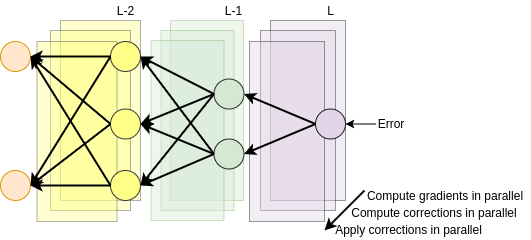
\includegraphics[scale=0.6]{fig/back_2.png}
	\caption{Backpropagation of the error. Each layer contains 3 parallel regions}
	\label{fig:back}
\end{figure}

\newpage

Similar to the forward propagation, we can associate operations to nodes, like computing the partial derivatives, and then, edges can be seen as streams, but this time, they transport the gradients in the opposite direction, from the last layer to the first one. Therefore the backpropagation phase could be considered also a task parallelism model.

Behind a NN, for both forward and backward propagation steps, there lie multiple regions with nested \textit{for} loops, so for this reason, the parallelization using \textit{openmp} is quite intuitive and easy.

In my code there are several simple \textit{for} loops(non-nested) and I chose to keep them sequential, as they do not go over large array(like number of neurons in a layer), so their parallelization would not produce significant time improvement.

\newpage




	
\begin{itemize}

\item	Give a brief overview of the overall algorithm (what is the algorithm you are parallelizing?)
	
\item	Identify where parallelism can be introduced to the algorithm
	
\item	Discuss the code executed by the master and the slaves
	
\item	Discuss how the master and slaves communicate and why they communicate
	
\item	Provide figures and equations to support your explanations
	
\item	There should be no results in this section
	
\item	After reading this section, we should have a complete understanding of how you solved the problem without having to read your code for further details.
	
\item	At the same time, there should be little to no code in your report.
\end{itemize}	
	\section{Results/Data Analysis}
	Include all necessary tables (and make sure they are completely filled out)
	
	Include all relevant figures
	
	Introduce all tables and figures in text BEFORE they appear in the report
	
	When answering questions, always provide explanations and reasoning for your answers.
	
	If you don't know what a question or requirement is asking for, please ask us in advance! We are here to help you learn.
	
	
	\section{Conclusion}
	Restate the purpose or objective of the assignment
	
	Was the exercise successful in fulfilling its intended purpose?
	
	Why was it (or wasn't it)?
	
	Summarize your results
	
	Draw general conclusions based on your results (what did you learn?)
	
	
	
	
	%\begin{table}[h!]
	%	\begin{center}
	%		\begin{tabular}{|c | c | c | c | c | c | c |} 
	%			\hline
	%			Population & Time & Type & Start\_pos& End\_pos& Mutation & Mutation category\\ [0.5ex] 
	%			\hline\hline
	%			1 & 30000 & INS & 114034 & 114034 & (C)6$\rightarrow$7 & small\_indel \\ [0.5ex]  \hline
	%			8 & 10000 & DEL & 114034 & 114034 & (C)6$\rightarrow$5 & small\_indel\\ [0.5ex]  \hline
	%		\end{tabular}
	%		\caption{Mutations that may be the reason for increased mutation rates}
	%		\label{mutT_mut}
	%	\end{center}
	%\end{table}
	
	
	
	%\begin{figure}[htbp]
	%	\centering
	%	\subfloat[Population 1]{
	%		\includegraphics[scale=0.7]{pop_1.png}
	%		\label{fig:img1} } \hspace*{-1.7em}
	%	\subfloat[Population 2]{
	%		\includegraphics[scale=0.5]{pop_2_v2_green.png}
	%		\label{fig:img2} } \\
	%	\caption{Mutations from the last generation that occur at previous timepoints}
	%	\label{fig:ancestor_mut}
	%\end{figure}
	
	
	
	
	\newpage
	
	\bibliographystyle{plain}
	\bibliography{bibliography}
	
	
	
\end{document}
